\chapter{The Standard Model of Particle Physics}\label{ch:sm}

The Standard Model is a set of theories describing the interactions between elementary particles.
It explains three of the four known fundamental forces, namely the electromagnetic force,
the weak nuclear force, and the strong force.
It does not include  or account for gravitational interactions.

The Standard Model can be fairly characterized as one of the most successful theories in science.
A huge number of predictions made by the theory have been confirmed experimentally,
some to an astounding degree of accuracy.
Precision measurements of the magnetic moment of the electron have shown the experimental and theoretical values of the
fine structure constant to agree better than one part in one billion.\cite{sm-fine-structure-2008}
The ATLAS detector at the LHC has confirmed the predicted rate of particle production for a very wide range of
production processes and final states.
A summary of Standard Model measurements made by ATLAS, and their comparisons to theoretical predictions can be seen in figure~\ref{fig:sm_xsec_summary}.
The Standard Model predicted the existence of the W boson, the top quark, and the Higgs boson,
which were all later confirmed by experiment.

\begin{figure}[h]
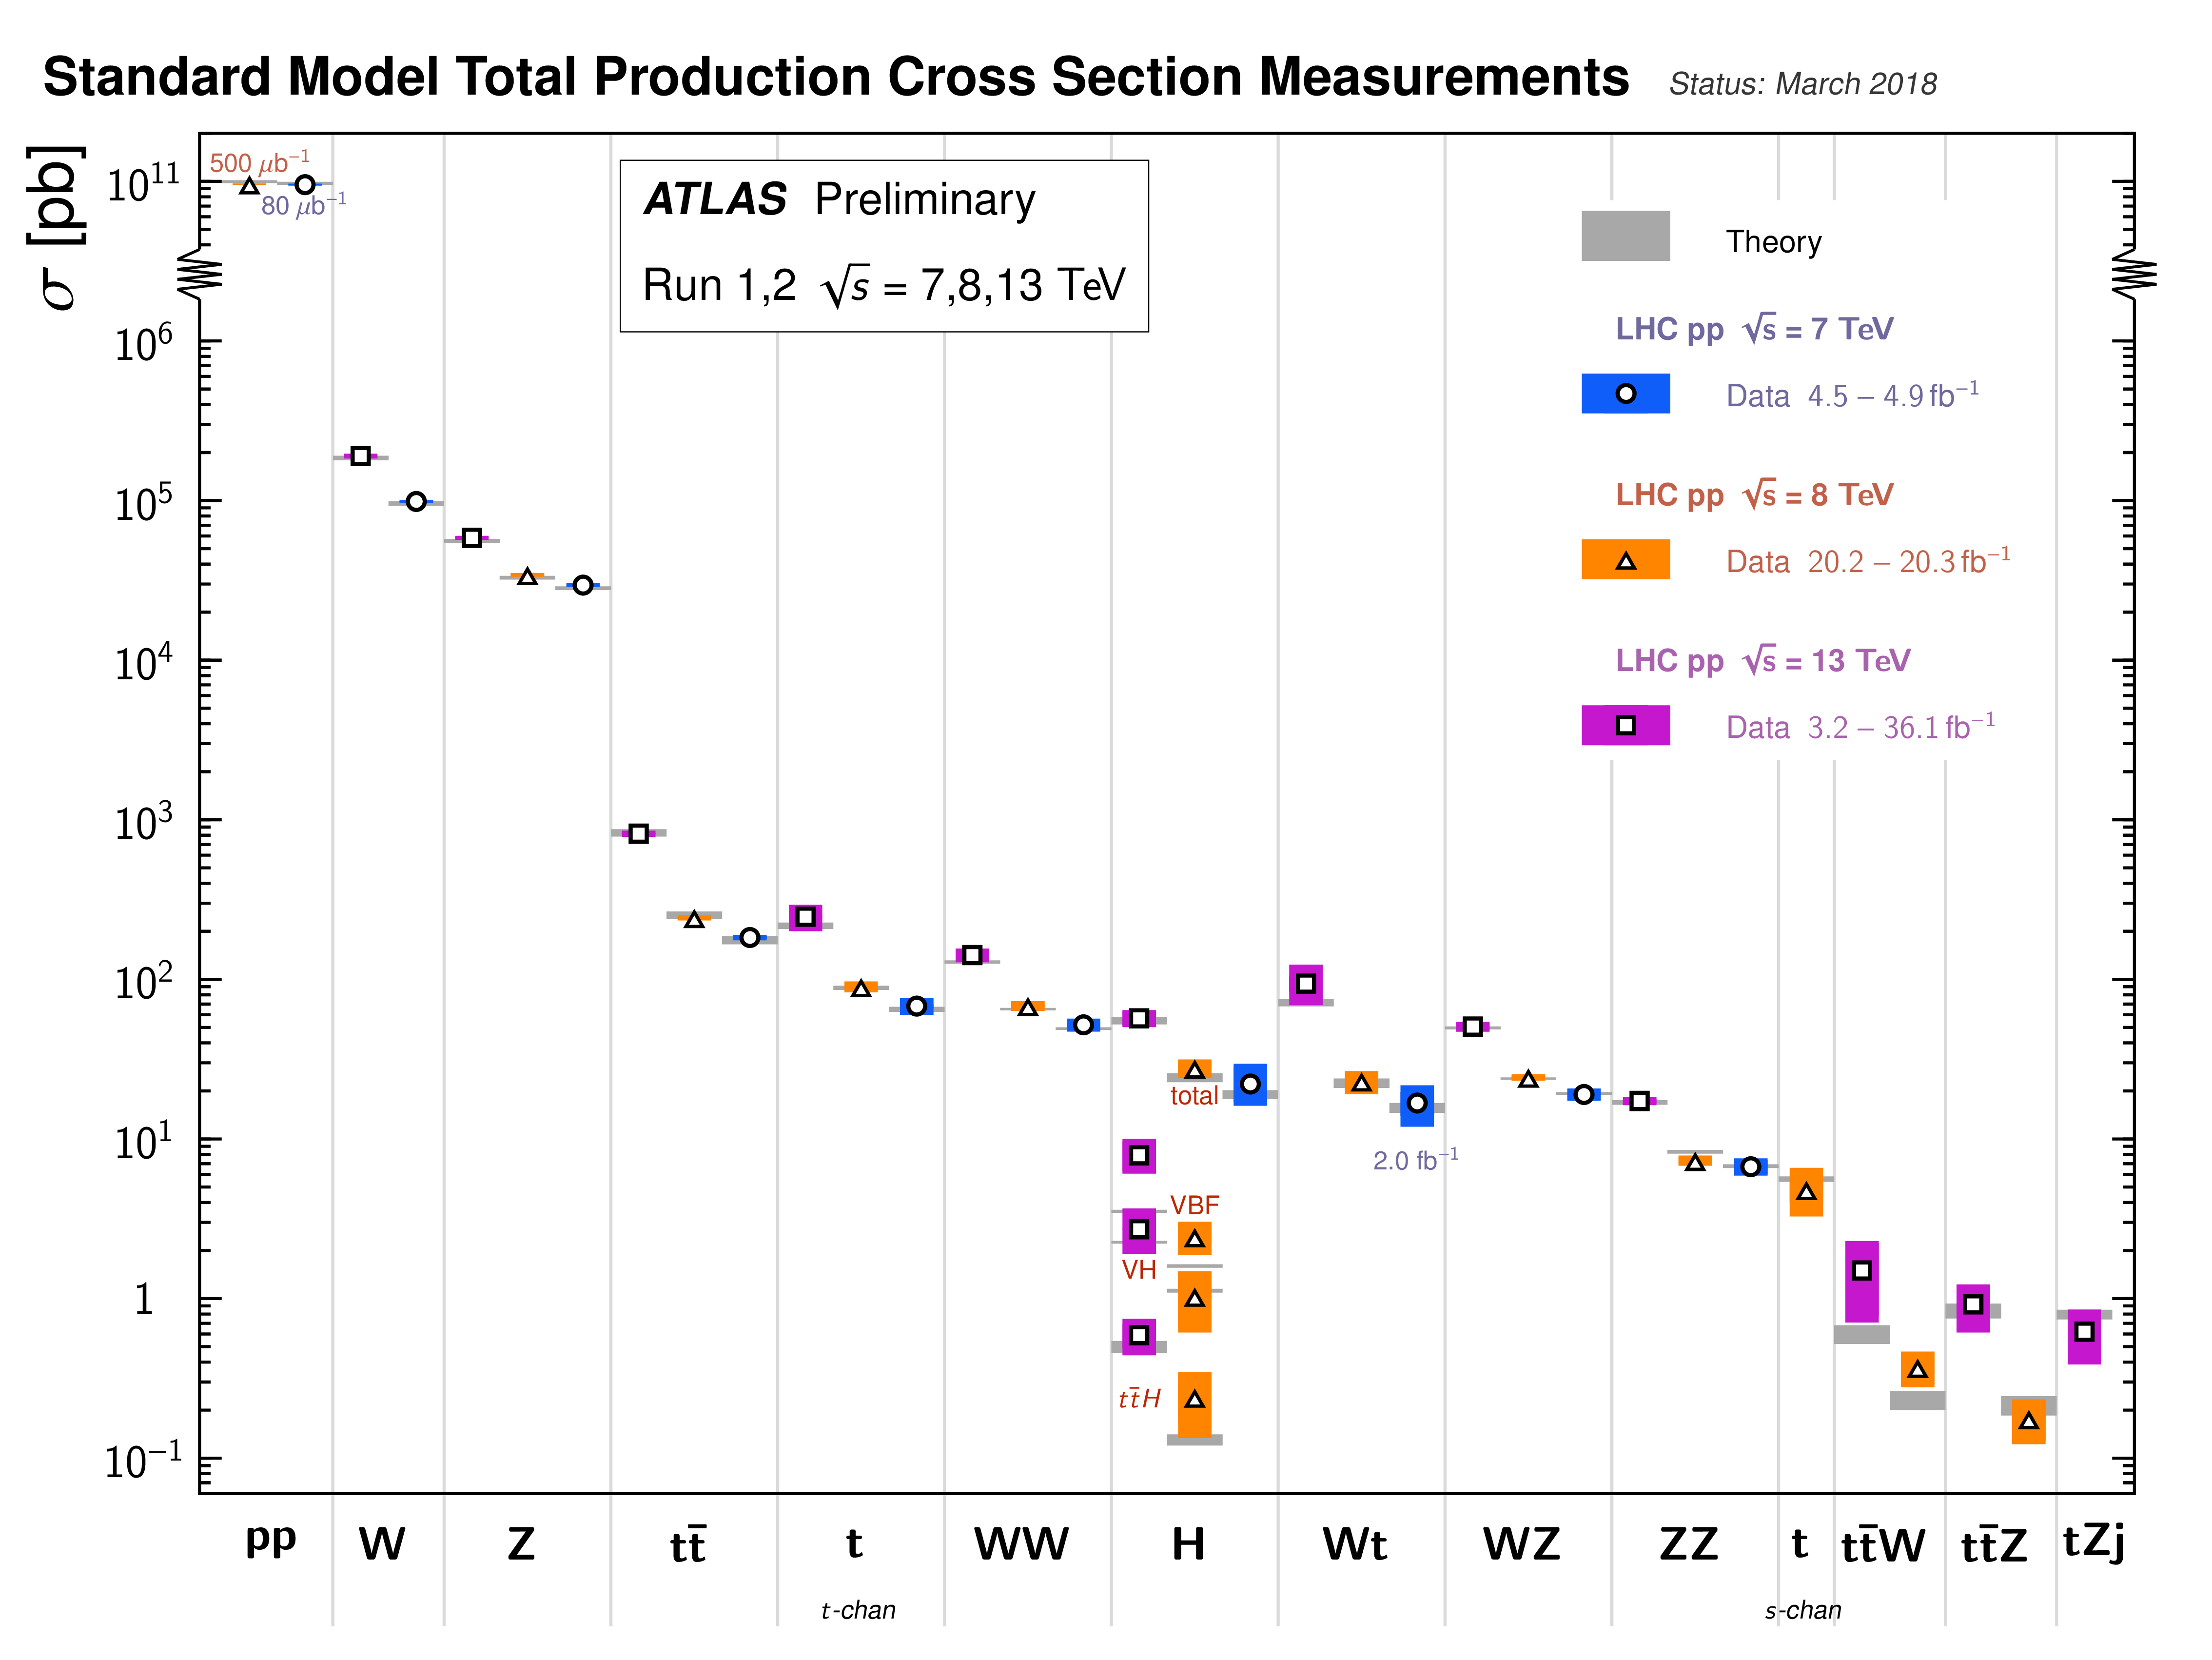
\includegraphics[width=\textwidth]{sm_xsec_summary}
\caption{Summary of Standard Model proudction cross sections measured by ATLAS, compared to theoretical predictions.}
\label{fig:sm_xsec_summary}
\end{figure}

The Standard Model is expressed in the language of Quantum Field Theory.
The theory consists of three generations of matter fields,
specified by their representation under the gauge group $SU(3)\times SU(2)\times U(1)$ and the Lorentz group,
as well as a complex scalar field.

The Standard Model is a complete theory in the sense that it is internally self-consistent,
and all particles predicted by the theory have been discovered experimentally.
However, the Standard Model does not account for all known physical phenomena,
and so cannot be considered a complete theory of nature.

\section{Electroweak Symmetry Breaking}\label{sec:sm_ew}

The Lagrangian describing the electroweak sector of the Standard Model is:

\begin{equation}\label{eq:ew_lagrangian}
    \mathcal{L} =
\end{equation}

\section{Quantum Chromodynamics}\label{sec:sm_qcd}

\section{Phenomenology}\label{sec:sm_pheno}

\section{Limitations}\label{sec:sm_limits}
